\chapter{Przetwarzanie heterogeniczne}\label{cha:hpo}

%---------------------------------------------------------------------------

\section{Wprowadzenie}\label{sec:wprowadzenie}


Lata 50-te XX wieku były przełomowym okresem w dziedzinie elektronicznego przetwarzania danych. Opracowana w 1945 roku \emph{Architekura von Neumana}~\cite{b16} pozwoliła na uruchomienie pierwszych komputerów ogólnego przeznaczenia. Mimo, że \emph{Architektura Harwardzka}~\cite{b17} została opracowana 6 lat wcześniej, \emph{Architektura von Neumana} była łatwiejsza w implementacji przez przechowywanie danych wraz z programem na jednej wspólnej pamięci. Pierwszym komputerem opartym na pomyśle Neumana, który wykonywał instrukcje zapisane w fizycznej pamięci, był powstały w 1948 roku Small-Scale Experimental Machine. Stał się on bazą do rozwijania kolejnych urządzeń. W ten sposób w 1949 roku powstał EDSAC (akronim od ang. Electronic Delay Storage Automatic Calculator). Został uznany jako  pierwszy komputer wykorzystywany w praktyce do obliczeń naukowych. EDSAC rozbudowany był o dodatkowe układy peryferyjne. W celu odczytu danych zastosowano w nim dalekopis – aparat drukujący dane w postaci alfanumerycznej. Skonstruowanie komputerów zerowej, pierwszej i drugiej generacji znacznie rozwinęło moc obliczeniową tych urządzeń. W dalszym ciągu jednak stosowano niewygodne formy prezentacji danych – wyświetlacze złożone z szeregu lamp, perforowane karty. W 1975 roku, w jednym z pierwszych komputerów osobistych IBM 5100, zastosowano kineskopowy wyświetlacz, który mógł wyświetlać 16 linii po 64 znaków. 6 lat później, w kolejnym modelu IBM 5150, wprowadzono możliwość instalacji kart rozszerzeń ISA. Zastosowano w nim pierwszą kartę graficzną Monochrome Display Adapter (MDA). Rozpoczęło to rozwój peryferyjnych układów komputera, które stały się niezależnymi platformami z własnym procesorem i pamięcią. Początkowo karty graficzne były w stanie wyświetlać jedynie znaki alfanumeryczne przechowywane w pamięci karty. Kolejne generacje kart pozwalały na rysowanie obrazów przy użyciu pojedynczych pikseli, a nowoczesne układy graficzne pozwalały na akcelerację 2D i 3D, korzystając z wbudowanych funkcji do generowania obrazu. W najnowszych procesorach grafiki umożliwiono użytkownikowi zaprogramowanie ich w dowolny sposób. Charakterystyka obliczeń przy przetwarzaniu obrazów wymusiła architekturę procesorów graficznych w postaci dużej ilości jednakowych jednostek ALU (ang. Arithmetic Logic Units), potrafiących wykonać równolegle wiele prostych operacji (Rys. 3.1.).
\begin{figure}[h]
        \centering
                \centering
                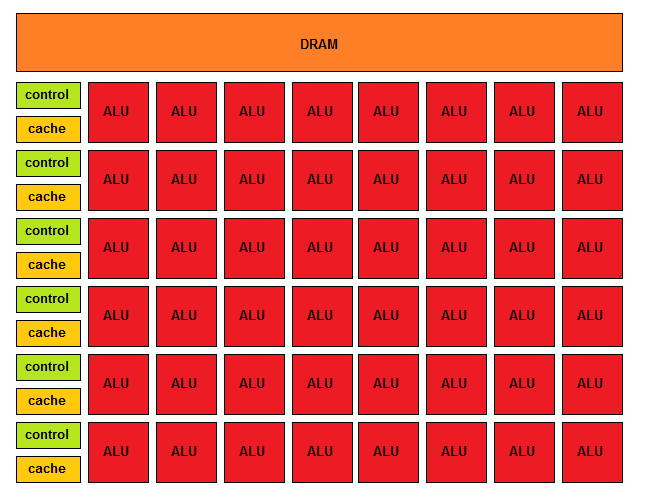
\includegraphics[width=12cm]{rys7}
	\caption{Architektura procesora GPU.}
\end{figure}
Taka budowa kart graficznych pozwoliła na wykorzystanie ich nie tylko do obliczeń związanych z generowaniem grafiki, ale także innych obliczeń przetwarzania danych, co doprowadziło do powstania kart ogólnego przeznaczenia (GPGPU).



%---------------------------------------------------------------------------

\section{Heterogeniczne platformy obliczeniowe}\label{sec:hetero}

Początkowo GPGPU były wykorzystywane do zaawansowanego generowania grafiki. Dążenie do realizmu w grach komputerowych rozwinęło karty graficzne o algorytmy wymagające przetwarzania równoległego, takie jak shading~\cite{b18} czy ray-tracing~\cite{b3}. W celu odciążenia procesora od złożonych obliczeń, na kartach graficznych zaczęto implementować fizykę obiektów – obliczenia związane z mechaniką klasyczną, symulacje zachowania cieczy, zachowania układów ciągłych i inne efekty cząsteczkowe. Dla ułatwienia programistom wykorzystania możliwości GPGPU, NVIDIA w 2007 roku wprowadza platformę CUDA. Jest to środowisko programistyczne i biblioteka umożliwiająca wykorzystanie kart graficznych produkowanych przez firmę NVIDIA. Umożliwia ona pisanie kodu opartego na C/C++ wykonywanego na procesorze karty i mającego bezpośredni dostęp do jej pamięci. Ułatwienie implementacji algorytmów na GPGPU rozwinęło wykorzystywanie tych kart w różnych dziedzinach naukowych, takich jak kryptografia, fizyka kwantowa, ekonomia czy medycyna. Wykonywanie  skomplikowanych obliczeń przy użyciu CUDA stało się powszechne na komputerach domowych, ale było ograniczone przez wymagania sprzętowe. 2 lata po wprowadzeniu CUDA firma Apple Inc wprowadza OpenCL (ang. Open Computing Language). W przeciwieństwie do produktu NVIDA, OpenCL umożliwia pisanie programów na heterogeniczne platformy – układy złożone z różnego rodzaju procesorów. Daje to możliwość pisania aplikacji na komputery z układami większości popularnych producentów, lub  na dowolne układy złożone z różnych procesorów (m. in. CPU, GPU, DSP, FPGA), oraz zapewnia przenośność programów.

%---------------------------------------------------------------------------

\section{Modele obliczeń równoległych}\label{sec:Paralellism}

Obliczenia równoległe to typ obliczeń komputerowych, w których wiele instrukcji wykonywanych jest jednocześnie~\cite{b14}. Złożone problemy często mogą być rozłożone na mniejsze zadania, które mogą być wykonywane w tym samym czasie. Daje to możliwość szybszego rozwiązywania problemów bez zwiększania częstotliwości taktowania procesora. W uproszczeniu energia wydzielana przez procesor, a w większości ciepło, wzrasta wraz z kwadratem częstotliwości taktowania. Ze względu na te fizyczne ograniczenia procesora wielordzeniowe procesory i obliczenia równoległe stały się dominującym paradygmatem architektury komputerów.

Obliczenia równoległe dzielą się na cztery różne modele:

- równoległość bitów

- równoległość instrukcji

- równoległość danych

- równoległość zadań.\\

Modele obliczeń równoległych mogą być implementowane oddzielnie lub w połączeniu ze sobą.

\subsection{Równoległość bitów}\label{sec:bitp}

Równoległość na poziomie bitów jest modelem przetwarzania równoległego opartym na zwiększaniu ilości bitów w pojedyńczym słowie procesora. Zwiększenie pojemności słowa zmniejsza liczbę instrukcji, które procesor musi wykonać, aby wykonać operację na zmiennych o rozmiarach większych niż długość słowa.
Początkowo komputery opierały się na jednobitowych procesorach. Pierwszym nieszeregowym komputerem był 16-bitowy Whirlwind z 1951 roku. Obecnie w komputerach osobistych funkcjonuje standard 32 i 64-bitowych architektur procesorów i systemów operacyjnych. Większa szerokość słowa wymagałaby znacznie większej zewnętrznej szyny danych, co jest kosztowne do wykonania przy obecnych procesach technologicznych. 64-bitowe słowo w większości jest wystarczające do  procesowania zmiennych wykorzystywanych na komputerach osobistych. Przy złożonych obliczeniach inżynierskich duże dane przechowuje się na kilku zmiennych i przetwarza przy użyciu kilku instrukcji procesora.

\subsection{Równoległość instrukcji}\label{sec:instp}

Równoległość na poziomie instrukcji jest oparta na równoległym wykorzystaniu kilku jednostek wykonawczych procesora. Większość procesorów składa się z kilku jednostek arytmetyczno-logicznych ALU, odpowiadających za wykonywanie operacji arytmetycznych i logicznych przez procesor oraz kilku jednostek zmiennoprzecinkowych FPU, odpowiadających za wykonywanie operacji arytmetycznych na liczbach zmiennoprzecinkowych. Wszystkie jednostki ALU i FPU mogą wykonywać operacje równolegle. Przykładowo, w poniższym kodzie (Kod ...), operacja z linijki 4 może być wykonana na jednostce ALU, a operacja z linijki 5 na jednostce FPU. Wykorzystując równoległość na poziomie instrukcji obie operacje mogą być wykonane przy użyciu jednej instrukcji procesora.

\begin{program}
\caption{Plik wejściowy programu}
\begin{lstlisting}
float a = 1.0, b = 2.0, c;
int x = 1, y = 2, z, w;

c = a + b;
z = z * y;
\end{lstlisting}
\end{program}

W zależności od architektury komputera, rozdzielenie operacji na jednostki wykonawcze procesora może być wykonane dynamicznie w trakcie wykonywania programu lub statycznie na poziomie kompilacji. Dynamicznie ustawiana równoległość instrukcji wykorzystywana jest w powszechnie dostępnych procesorach CPU. Zwiększa ona szybkość wykonywania programu oraz odciąża programistę i kompilator od procesu rozdzielenia instrukcji. Rozmieszczenie instrukcji na etapie kompilacji wykorzystywane jest w procesorach DSP i GPU. Pozwala to optymalizację kodu przed jego wykonaniem i obliczenie dokładnego czasu w jakim program będzie się wykonywał.  

\subsection{Równoległość danych}\label{sec:datap}

Równoległość na poziomie danych wykorzystywana jest przy obliczeniach na dużych zbiorach danych, gdzie obliczenia dla pojedyńczych danych są od siebie niezależne. W tym modelu zbiór danych dzielony jest na mniejsze zbiory i definiowany jest zestaw zadań, które zostaną wykonane dla pojedyńczego zbioru. Mniejsze zbiory danych wysyłane są do oddzielnych jednostek sterujących, które wykonują na nich równolegle zdefiniowany zestaw zadań. Równoległość danych jest najwydajniejsza dla dużych zbiorów podobnych danych (np. wektory, macierze), dla prostych operacji takich mnożenie macierzy, transformata Fouriera. Szybkość wykonywania programu opartego na tym modelu zależy od ilości jednostek sterujących, dlatego paralelizm danych często implementowany jest na procesorach graficznych, gdzie ilość tych jednostek sięga kilku tysięcy.

\subsection{Równoległość zadań}\label{sec:taskp}

Równoległość na poziomie zadań to model, gdzie równolegle wykonywane są różne zadania na tych samych lub różnych zbiorach danych. Najczęściej wykorzystywany jest na wielordzeniowych procesorach CPU, gdzie każdy rdzeń może wykonywać bardziej złożone operacji niż w przypadku modelu równoległości danych. Rozdzielenie zadań pomiędzy rdzenie wykonywane jest na poziomie pisania kodu aplikacji lub obsługiwane przez system operacyjny. Większość współczesnych systemów operacyjnych wykorzystuje równoległość zadań do wykonywania procesów na oddzielnych wątkach.

%---------------------------------------------------------------------------

\section{Środowisko OpenCL}\label{sec:OpenCL}

OpenCL~\cite{b21} jest platformą programistyczną opracowaną w 2009 roku przez Apple Inc, a następnie utrzymywaną przez Khronos Group. Umożliwia programowanie heterogenicznych układów procesorowych w języku opartym na C99 i C++11. Wykorzystanie OpenCL nie ogranicza się jedynie do procesorów graficznych. Jego główną zaletą jest przenośność na większość popularnych procesorów CPU, DSP, a nawet układów FPGA. Każdy procesor z instrukcjami SSE2 może zostać wykorzystany jako urządzenie OpenCL. Standard OpenCL dostarcza interfejs programistyczny (API), biblioteki dla wielu popularnych języków programowania oraz sterowniki do urządzeń.

\subsection{Platforma}\label{sec:platforma}

Aplikacja pisana w OpenCL opiera się na jednostkach zwanych platformami. Każda platforma odpowiada za przygotowanie danych do obliczeń i rozdzielenie zadań. W nowszych standardach kod platformy może być pisany w wielu popularnych językach  (m. in. Python, Matlab). Każda platforma zawiera kontekst, w którym definiowane są dane wejściowe, kolejka zadań i urządzenia do wykonywania obliczeń. Każde urządzenie zawiera jednostki obliczeniowe (ang. compute units, CU), które składają się z elementów przetwarzania (ang. processing elements, PEs)(Rys. 3.2.). 

\begin{figure}[h]
        \centering
                \centering
                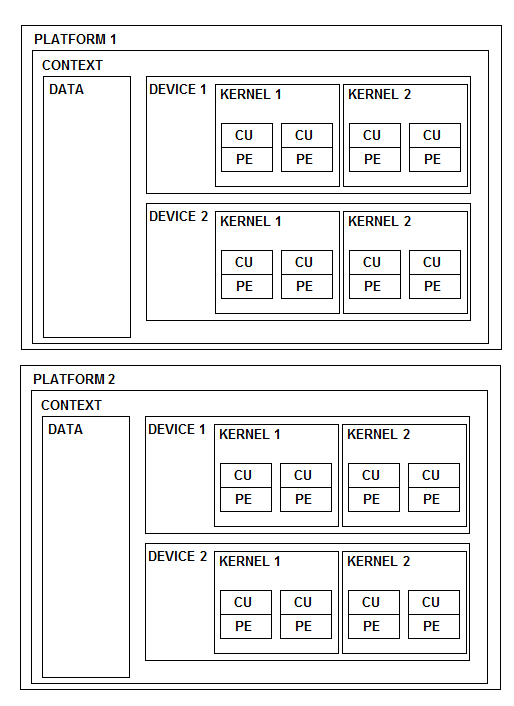
\includegraphics[width=12cm]{rys8}
	\caption{Architektura programu napisanego w bibliotece OpenCL.}
\end{figure}

Pojedyńcza platforma odnosi się do poszczególnego sterownika. Przykładowo na komputerze z procesorem Intel i kartą graficzną AMD mozemy uruchomić dwie platformy, jedną dla OpenCL™ Runtimes for Intel® Processors~\cite{b22} i drugą dla wyspecjalizowanego sterownika AMD dla danej karty graficznej. Każda platforma może obsługiwać więcej niż jedno urządzenie, w szczególnych przypadkach może zawierać złożone układy kart graficznych. 

Standard OpenCL definiuje obsługę mieszanych wersji platform (ang. Platform Mixed Version Support). Oznacza to, że w jednej aplikacji możemy użyć różnych wersji platform, urządzeń i języka OpenCL. Domyślnie standard używa najnowszej wersji języka dostępnej na danym urządzeniu.

\subsection{Model wykonywania programu}\label{sec:mwp}

Wykonywanie programu OpenCL następuje w dwóch krokach: uruchomienie kodu głównego na urządzeniu gospodarza i wykonywanie kodu kernela na urządzeniach OpenCL. Kod gospodarza definiuje platformy i zarządza wykonywaniem kerneli. Dla każdego kernela definiowana jest przestrzeń indeksowania. Każdy element przestrzeni indeksowania jest unikalnym identyfikatorem i dla każdego z nich wykonywany jest kod kernela. Instancję kernela wywołaną w obrębie jednego indeksu nazywamy wątkiem (ang work-item). Każdy wątek wykonuje ten sam kod, ale jego działanie może zależeć od przydzielonego mu indeksu. Posługując się identyfikatorem z przestrzeni indeksowej możemy dla każdego wątku wybrać inny zakres danych do obliczeń lub wykonać inny typ obliczeń. Ta własność, w połączeniu z możliwością wykonywania różncych kerneli w jednej aplikacji, umożliwia pisanie programów zarówno w modelu równoległości danych, jak i modelu równoległości zadań.

\subsection{Przestrzeń indeksowania}\label{sec:OpenC5L}

Przestrzeń indeksowania w standardzie OpenCL definiowana jest przez typ NDRange. Jest to jedno-, dwu- lub trójwymiarowa tablica liczb całkowitych. Cała przestrzeń dzieli się na grupy o takim samym wymiarze jak wymiar całej przestrzeni (ang. work-groups). Każdy wątek może być zidentyfikowany po jego globalnym indeksie lub po kombinacji indeksu grupy i lokalnego indeksu wewnątrz grupy. Wątki wewnątrz jednej grupy wykonywane są na jednym elemencie przetwarzania. Podział na grupy może być zrealizowany ze względu na ilość jednostek przetwarzania lub charakter obliczeń. Przestrzeń ideksowania stanowią rosnące wartości liczb całkowitych z zadanym przesunięciem, więc może ona reprezentować indeksy wektora, macierzy lub dziedzinę funkcji.

\subsection{Kontekst obliczeniowy}\label{sec:OpenC2L}

Definiowany na urządzeniu gospodarza na pojedyńczej platformie kontekst obliczeniowy odpowiada za przygotowanie następujących zasobów:

- Urządzenia OpenCL - zbiór urządzeń podpiętych pod urządzenie gospodarza, na których wykonywane są kernele.

- Kernele - funkcje napisane w języku OpenCL, które wykonywane są na poszczególnych urządzeniach.

- Obiekty programu - źródła i pliki wykonywalne programu gospodarza.

- Obiekty pamięci - przestrzeń pamięci na urządzeniu gospodarza, w której przechowywane są dane wejściowe i wyjściowe wykonywania kernela.\\

Kontekst pisany jest zgodnie z interfejsem OpenCL, który udostępnia kolejkę zadań (ang. command-queue). Kolejka zadań zawiera listę zadań do wykonania, które postępują asynchronicznie względem urządzenia gospodarza. Zadaniami mogą być:

- Zadanie wykonania kernela - wykonanie kernela na konkretnym elemencie przetwarzania na konkretnym urządzeniu.

- Zadanie pamięci - przeniesienie danych pomiędzy pamięcią gospodarza, a pamięcią urządzenia, lub przekazanie wskaźnika na adres pamięci gospodarza do urządzenia.

- Zadanie synchronizacji - wymuszenie kolejności wykonywania zadań z kolejki.\\

Wykonywanie zadań z kolejki może być wykonywane w kolejności (ang. In-order execution) lub poza kolejnością (ang. Out-order execution). W pierwszym wariancie kolejne zadanie z kolejki może być wykonywane dopiero po zakończeniu poprzedniego zadania. Zadanie wykonywane poza kolejnością rozpoczyna działanie przed zakończeniem poprzedniego zadania. Synchronizacja pomiędzy zadaniami jest wykonywana przez programistę wykorzystując komendy synchronizacyjne z interfejsu OpenCL.

W jednym kontekście może być zdefiniowana więcej niż jedna kolejka. Takie kolejki wykonywane są jednocześnie i niezależnie. Standard OpenCL nie udostępnia mechanizmu dedykowanego do synchronizacji pomiędzy kolejkami.


\subsection{Kernel}\label{sec:OpenC4L}

Funkcja kernela jest kodem napisanym w języku OpenCL wykonywanym na urządzeniu OpenCL. Zdefiniowa jest poprzez kwalifikator \verb|__kernel|. Język kernela oparty jest na C99 i C++11 i w zależności od wersji OpenCL może wykorzystywać niektóre funkcje biblioteczne z tych języków. Przykładowo od wersji OpenCL 1.2 w kodzie kernela możliwe jest użycie funkcji printf.

Rozróżniane są dwa typy kerneli:

- Kernele OpenCL - napisane w języku OpenCL C i skompilowane przy użyciu kompilatora OpenCL.

- Natywne kernele - funkcje skompilowane przez inny kompilator niż OpenCL. Najczęściej są to funkcje wyeksportowane z zewnętrznych bibliotek.\\

Kod kernela kompilowany jest do obiektu kernela podczas wykonywania kodu głównego na urządzeniu gospodarza. Zbudowanie obiektu kernela wytwarza program oparty na jego kodzie i powiązany z przypisanymi mu danymi wejściowymi. Dane wejściowe mogą być przekazane do kernela w postaci wskaźnika na adres pamięci urządzenia gospodarza lub przeniesione do lokalnej pamięci urządzenia. Formy przekazywania pamięci i jej typy przedstawione są w rozdziale 3.4.8.

\subsection{Urządzenia OpenCL}\label{sec:OpenC21L}

Urządzenie OpenCL stanowi interfejs do zbioru jednostek obliczeniowych. W generalnym przypadku są to karty GPU, wielordzeniowe procesory CPU, DSP i procesory typu Cell/B.E.

Standard OpenCL udostępnia 5 różnych rodzajów urządzeń:

- \verb|CL_DEVICE_TYPE_CPU| - urządzenie gospodarza na którym, oprócz kodu głównego, mogą być wykonywane kernele.

- \verb|CL_DEVICE_TYPE_GPU| - urządzenie GPU podłączone pod urządzenie gospodarza.

- \verb|CL_DEVICE_TYPE_ACCELERATOR| - dowolne urządzenie peryferyjne wspierane przez standard OpenCL.

- \verb|CL_DEVICE_TYPE_DEFAULT| - dowolne urządzenie dostępne na danej platformie.

- \verb|CL_DEVICE_TYPE_ALL| - wszystkie dostępne urządzenia dostępne na danej platformie.\\

Przy użyciu typu urządzenia możemy pobrać uchwyty do wybranych urządzeń dostępnych na platformie. Pobrane urządzenia mogą być przekazane do kontekstu gdzie definiowane jest ich użycie. Platforma OpenCL umożliwia pobranie informacji o urządzeniu takich jak typ urządzenia czy ilość jednostek obliczeniowych i elementów przetwarzania. Pozwala to na planowanie podziału danych, grup i przestrzeni indeksowania na poziomie pisania kodu i dynamiczne przydzielanie tych wartości w czasie wykonywania programu w zależności od urządzeń, na jakich jest on wykonywany.
 
\subsection{Jednostki obliczeniowe i elementy przetwarzania}\label{sec:OpenC3L}

Jednostki obliczeniowe (ang, Compute Unit, CU) i elementy przetwarzania (ang. Processing Element, PE) reprezentują różne fizyczne elementy procesora w zależności od jego rodzaju. Dla procesorów CPU CU jest równoważne PE i stanowi pojedyńczy rdzeń procesora. W kartach graficznych NVIDIA CU stanowi multiprocesor strumieniowy, a PE jego rdzenie. Karty graficzne AMD definiują CU jako jednostkę SIMD (ang. Single Instruction, Multiple Thread), a PE jako poszczególne linie jednostki SIMD. Na pojedyńczym elemencie przetwarzania wykonywany jest jeden wątek. Mimo że w zależności od urządzenia CU i PE reprezentują różne elementy procesora, odwołują się do nich w ten sam sposób. Umożliwia to wykonywanie programu gospodarza i kernela o jednakowej składni na różnych typach urządzeń. Kernele wykonywane są według kolejki zadań i rozdzielone pomiędzy jednostki obliczeniowe mogą być wykonywane równolegle na wielu elementach przetwarzania.

\subsection{Dostep do pamieci}\label{sec:OpenC6L}

OpenCL umożliwia dynamiczny dostęp do pamięci urządzeń oraz pamięci gospodarza. Każdy wątek ma dostęp do czterech typów pamięci:

- Pamięci globalnej – pamięci dostępnej przez wszystkie wątki w obrębie jednego kontekstu.

- Pamięć stałej – pamięci tylko do odczytu, dostępnej globalnie.

- Pamięci lokalnej – pamięci dostępnej w obrębie jednej grupy wątków.

- Pamięci prywatnej – pamięci dostępnej w obrębie jednego wątku.\\

Przepływ danych pomiędzy urządzeniem gospodarza a urządzeniem OpenCL może odbyć się poprzez operację kopiowania  lub odwzorowania z pamięci platformy do pamięci urządzenia. Rozmieszczenie typów pamięci i ich wzajemne relacje przedstawione są na Rysunku 3.2.

\begin{figure}[h]
        \centering
                \centering
                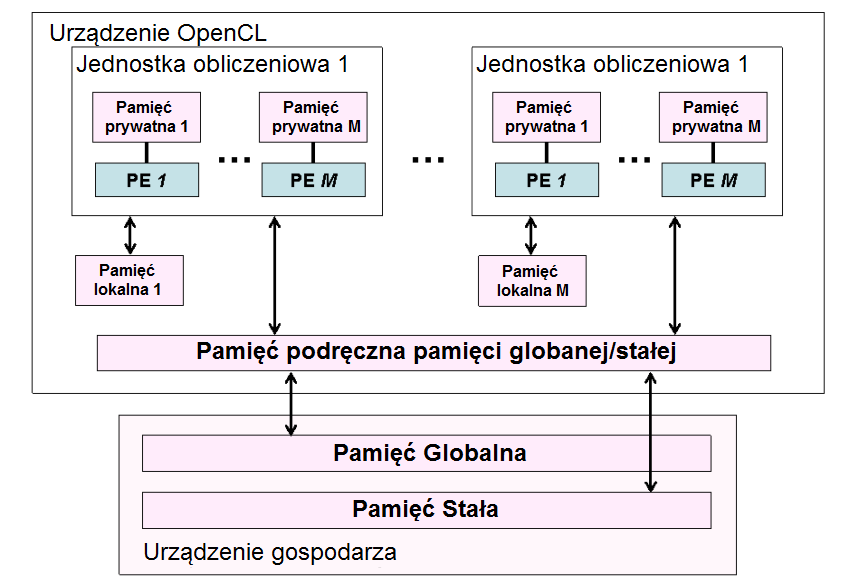
\includegraphics[width=12cm]{architekturapamieci}
	\caption{Architektura pamięciu na urządzeniach OpenCL.}
\end{figure}

Operacja kopiowania danych pomiędzy pamięcią gopodarza a pamięcią urządzenia jest wywoływana przez zadanie przeniesienia danych znajdujące się w kolejce zadań. Zadanie przeniesienia może być blokujące lub nieblokujące. Przeniesienie blokujące zabrania dostępu do pamięci urządzenia gospodarza aż do czasu zakończenia przenoszenia danych. Dostęp do pamięci urządzenia gospodarza przez wskaźnik na adres pamięci umożliwia modyfikację danych w tej pamięci przez wiele kerneli jednocześnie. Może to być wykorzystywane przy operacjach na wspólnym zbiorze danych takich jak funkcja splotu czy mnożenie macierzy.

Standard OpenCL opiera się na luźnym modelu spójności pamięci (ang. relaxed consistency memory model). Oznacza to, że stan pamięci widoczny przez poszczególne wątki nie jest spójny w każdej chwili. OpenCL gwarantuje spójność pamięci jedynie wewnątrz grupy. Spójność pamięci pomiędzy różnymi grupami musi być obsłużona poprzez punkty synchronizacji.

Dużym ograniczeniem wydajności obliczeń jest czas dostępu do pamięci. Pamięć o szerszym zakresie ma wolniejszy czas dostępu, dlatego najwydajniejsze obliczenia wykonują się dla niezależnych wątków działających równolegle na prywatnej pamięci.


\subsection{Synchronizacja}\label{sec:OpenC61L}

Istnieją dwie domeny synchronizacji w OpenCL:

- pomiędzy wątkami w obrębie jednej grupy,

- pomiędzy zadaniami z kolejki lub kolejek zadań w obrębie jednego kontekstu.\\

Synchronizacja pomiędzy wątkami w obrębie jednej grupy jest wykonywana przy użyciu bariery grupy (ang. work-group barrier). Wszystkie wątki z danej grupy muszą dojść do punktu bariery grupy zanim zacznie się wykonywanie programu poza barierą. Poprawne wykonanie programu jest możliwe tylko gdy wszystkie lub żaden wątek nie osiągnie bariery grupy. Standard nie udostępnia mechanizmu synchronizacji pomiędzy grupami.

Synchronizacja w obrębie kolejek zadań może odbywać przy użyciu dwóch mechanizmów:

- Bariera kolejki zadań. Bariera ta zapewnia, że wszystkie znajdujące się przed nią zadania w kolejce zostaną zakończone. Wszystkie obiekty pamięci, które są wykorzystywane przez późniejsze zadania, muszą zostać ustalone zanim zaczną się wykonywać zadania znajdujące się w kolejce po barierze. Bariera odnosi się tylko do jednej kolejki zadań i nie może być użyta do synchronizacji pomiędzy kolejkami. 

- Oczekiwanie na wydarzenie. Każda funkcja z interfejsu OpenCL, która kolejkuje zadania, zwraca wydarzenie identyfikujące to zadanie i wszystkie obiekty pamięci do których się odnosi. Dodatkowe zadanie w kolejce może czekać na wybrane wydarzenia z różnych zadań i stanowić punkt synchronizacji. Ten mechanizm może być użyty do synchronizacji pomiędzy kilkoma kolejkami.

\subsection{Obiekty pamięci}\label{sec:OpenC61asdL}

Obiekty pamięci przechowują dane, które mogą być przenoszone pomiędzy pamięcią urządzenia gospodarza a pamięcią urządzenia OpenCL. Obiekt pamięci jest obsługiwany przez typ \verb|cl_mem| i może być przekazany jako parametr wejściowy lub wyjściowy do funkcji kernela.

Standard definiuje dwa typy obiektów pamięci: bufor (ang. buffer object) i obraz (ang. image object). Obiekt bufora przechowuje jednowymiarowy zbiór elementów, natomiast obiekt obrazu może przechowywać dwu- lub trójwymiarowy zbiór elementów albo zbiór buforów. Podstawową różnicą między typami poza wymiarem jest ułożenie danych w pamięci. Elementy w buforze są ułożone w ciągłej pamięci i możemy się odwoływać do nich poprzez wskaźnik. Rozmieszczenie elementów obrazu nie jest widoczne dla użytkownika, a dostęp do nich odbywa się poprzez funkcje wbudowane w język OpenCL C. Elementami bufora mogą być dowolne typy danych obsługiwane przez język kernela, natomiast elementy obrazu stanowią czteroelementowe wektory liczb całkowitych lub zmiennoprzecinkowych. Stanowi to wygodny format do przechowywania plików graficznych. W przypadku przekazywania innego typu danych jako obraz, w funkcji kernela należy wykonać odpowiednią konwersję i interpretację danych.

%---------------------------------------------------------------------------

\section{Inne środowiska programowania heterogenicznego}\label{sec:others}

\subsection{CUDA}\label{sec:cuda}











